\documentclass[10pt, a4j]{jarticle}
\usepackage[english]{babel}
\usepackage{fed2012doc}
\usepackage{here}
\usepackage{amsmath}
\usepackage{placeins}
\usepackage[dvipdfmx]{graphicx}
\usepackage{fancyhdr}
\usepackage{indentfirst}
\usepackage{cite}
\usepackage[subrefformat=parens]{subcaption}

\title{\gt �l�̗͂�p�������{�b�g�̗U���Ɋւ��錤��\\%
{\normalsize \sf Study on robot guidance using human force}}
\author{%
Joshua SUPRATMAN, Chiba Institute of Technology\\
 $<$supratmanjoshua@gmail.com$>$ \\
}
\abstract{\fontsize{9}{10}\selectfont%
Abstract: In this paper, we present a method of attempting to induce a wheeled robotic manipulator using human force. We first discuss the orthodox method which we measure or estimate force applied on the manipulator to select a behavior. Next, we discuss the end-to-end method which estimates intension using reinforcement learning by directly taking sensor data as input and returning behavior as an output. We conduct our experiment on a simulator first before we conduct our experiment on the robot.
}
\keywords{\fontsize{9}{10}\selectfont%
Guidance, Reinforcement Learning, Intention Estimation, End-to-end Method
}

\twocolumn
\begin{document}
\maketitle

\section{Background}
Robots and human working in the same environment are increasing such as KAWADA Robotics NEXTAGE, a humanoid appearance manipulator design to perform tasks near human. Robots that are designed to work closely to human activity must consider, in addition to safety, how to convey information from human to robot. In general, this is usually done by sending command using an external controller; however this method does not always determine efficiency as it requires human to learn how to operate the robot beforehand. 

Intuitively, human have several means to communicate with each other such as visual and auditory communication. Physical communication is once such method. An example of physical communication would be a father guides their child by holding hands or a dog being pulled away on their leash by their owner. Communication through �eeffort�f or force is thought to be simpler method of communicating comparing to visual and auditory communication as learning feedback can directly occur without any prerequisite information unlike visual and auditory communication.

Using the same concept as above, this research attempts to mimic human's physical communication  on a robot by attempting to induce a wheeled robot with manipulator using human force as describe in figure \ref{fig:overview}.

\begin{figure}[!htbp]
\begin{center}
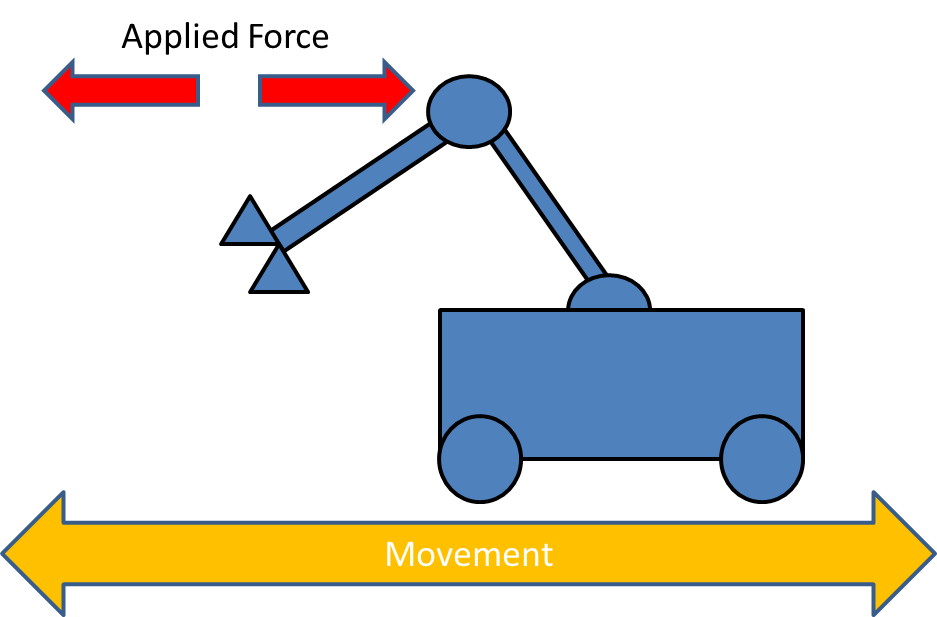
\includegraphics[width=7cm]{overview.png}
\caption{concept overview}
\label{fig:overview}
\end{center}
\end{figure}

\section{Related Works}
The concept of human robot interaction through physical communication was based on Professor Hayashiba�fs works \cite{haya} which uses orthodox method to accomplish this task.

Tohoku University have developed dance partner robot known as Ms DanceR \cite{kosuge}. The robot was developed with the goal of human-robot coordination with physical interaction.

Nextage Open is a machine learning based humanoid robot that was developed for production line worker \cite{yang}. The robot uses end-to-end method to accomplish human robot interaction using deep learning.

\section{Method of Measuring Force}
To guide the robot using human force, the orthodox method is to first estimate the force applied on the robot then executes a behavior as described in figure \ref{fig:orthodox}.

\begin{figure}[!h]
\begin{center}
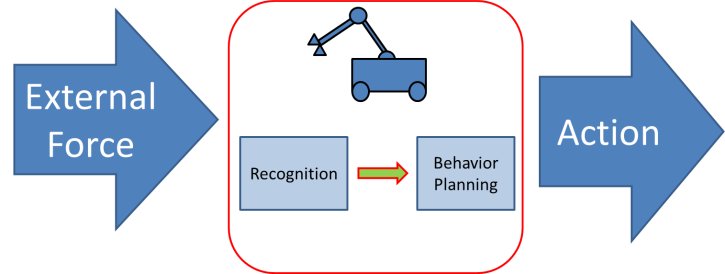
\includegraphics[width=9cm]{orthodox_method.png}
\caption{orthodox method}
\label{fig:orthodox}
\end{center}
\end{figure}

We attempted to estimate contact force on robotic manipulators in figure \ref{fig:manipulator}. There are two methods to measuring external force. 

\begin{enumerate}
\item Using force sensors to measure applied force.
\item Estimating applied force from joint torque. A common method is to use the current to find the torque as torque and current are proportional. Another method is using joint error positions to find the torque.
\end{enumerate}

\begin{figure}[!h]
\begin{center}
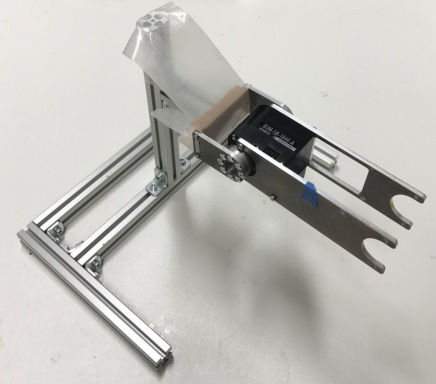
\includegraphics[width=5cm]{manipulator.jpg}
\caption{manipulator with a single DOF}
\label{fig:manipulator}
\end{center}
\end{figure}

Force sensors provide accurate measurement but cannot measure any force beyond their placement. On the other hand, estimating force from joint torque is difficult to obtain as estimation must also considered torque applied to hold the manipulator. 

There are limitations in using orthodox method. Measuring or estimating external force has a tradeoff between flexibility and accuracy. It is also difficult to write a rule for behavior selection for each joint state combination.

\section{Behavior Selection Through Reinforcement Learning}
Due to the challenges using orthodox method, in this paper, for robot to behave according to the applied force, we used reinforcement learning to estimate the intention of the applied force as describe in figure \ref{fig:end}. This method eliminates the need to recognize external force and plan behavior manually. Instead, we �etrain/teach�f the robot, in a manner similar to how father �etrain/teach�f their child, intuitively without scientific background requirement.

\begin{figure}[!h]
\begin{center}
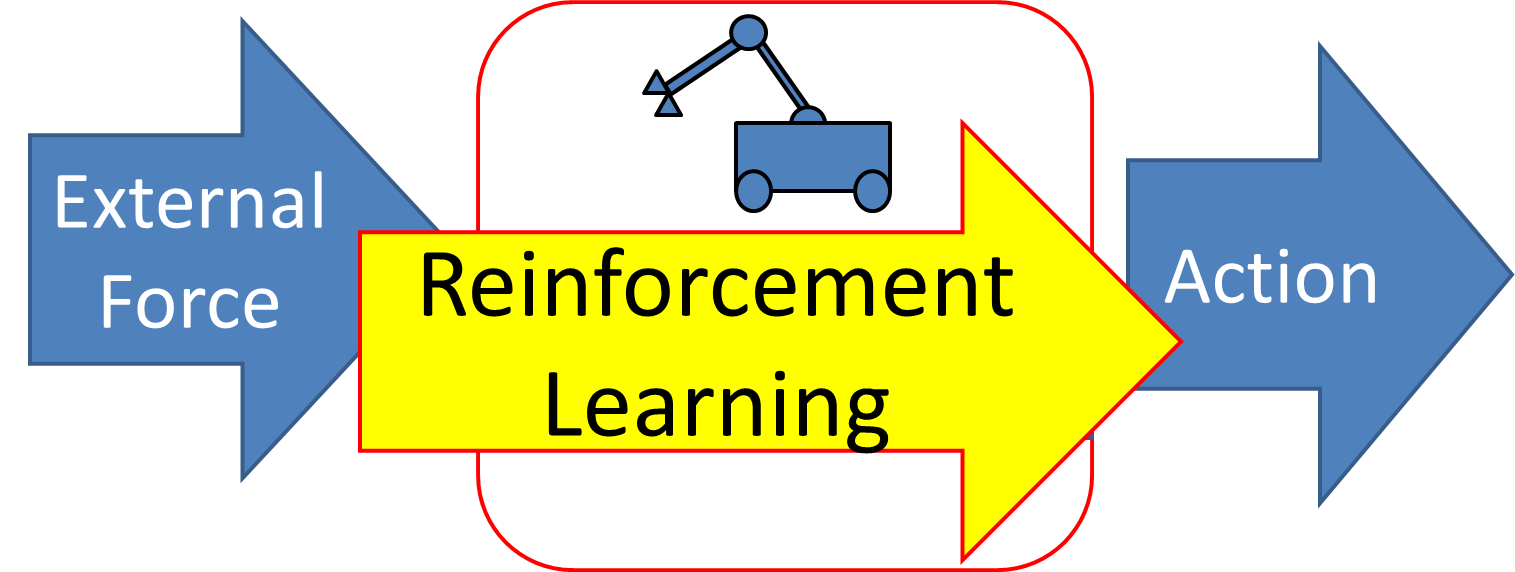
\includegraphics[width=9cm]{end_method.png}
\caption{end-to-end method}
\label{fig:end}
\end{center}
\end{figure}

Learning in reinforcement learning is accomplished by selecting behaviors to maximize the reward. Given the state $s$ in time step $t$, an agent seeks to execute action $a$ to maximize the reward $r$ which is define by $R_t=��_{\tau=t}^{��} \gamma^{\tau-t} r_\tau$ where $\gamma��[0,1]$ is a discount factor that trades-off priority of immediate and future rewards. Further introduction can be found in \cite{sutton}.

\subsection{Deep Q Network}
To handle high dimension input, this paper uses neural network to approximate using deep Q network \cite{mnih}, $Q(s,a;\theta)$ with parameters $\theta$ using the following Q-learning algorithm:

\begin{equation}
Target=r+\gamma maxQ(s',a';Q^{-})
\end{equation}

In reinforcement learning, approximating nonlinear function such as neural network are difficult to do as it is generally unstable and diverges. This however can be overcome using two key ingredient, experience replay and target network as describe in \cite{mnih}. \\

\subsection{Double Deep Q Network}
In this paper, it is planned to use the Double DQN (DDQN) reinforcement learning algorithm proposed by \cite{van}. The Q-Learning algorithm and the conventional DQN algorithm uses the max operators to estimate the true value. However, this tends to overestimates the optimal value as describe in \cite{van}. To overcome this problem, DDQN uses the following algorithm:
\begin{equation}
Target=r+\gamma Q(s',argmax(Q(s',a';\theta_{i});Q^{-})
\end{equation}
\section{Experiment Condition}
The environment for the experiment is shown in Table \ref{tab:environment} and figure \ref{fig:home}, \ref{fig:servo}, \ref{fig:model}. Table \ref{tab:network} shows the expected network model.

\begin{table}[!htbp]
\begin{center}
\caption{experiment environment}
\label{tab:environment}
\begin{tabular}{|c|c|}
\hline
Operating System & Ubuntu14.04 LTS \\
\hline
Middleware & ROS indigo \\
\hline
Hardware & @home robot \\
\hline
Input Actuator & KONDO B3M-SC1170-A \\
\hline
Output Actuator & TF-M30-24-3500-G15R \\
\hline
Simulator & Gazebo 7.1 \\
\hline
\end{tabular}
\end{center}
\end{table}

\begin{table}[!htbp]
\begin{center}
\caption{network model}
\label{tab:network}
\begin{tabular}{|c|c|c|}
\hline
Layers & No. of Nodes & Activation \\
\hline
Input & 6 (joint error positions) & Linear \\
\hline
Hidden 1 & 100 & ReLU \\
\hline
Hidden 2 & 100 & ReLU \\
\hline
Output & 3 (forward, stop, reverse) &  \\
\hline
\end{tabular}
\end{center}
\end{table}

\begin{figure}[!htbp]
\begin{center}
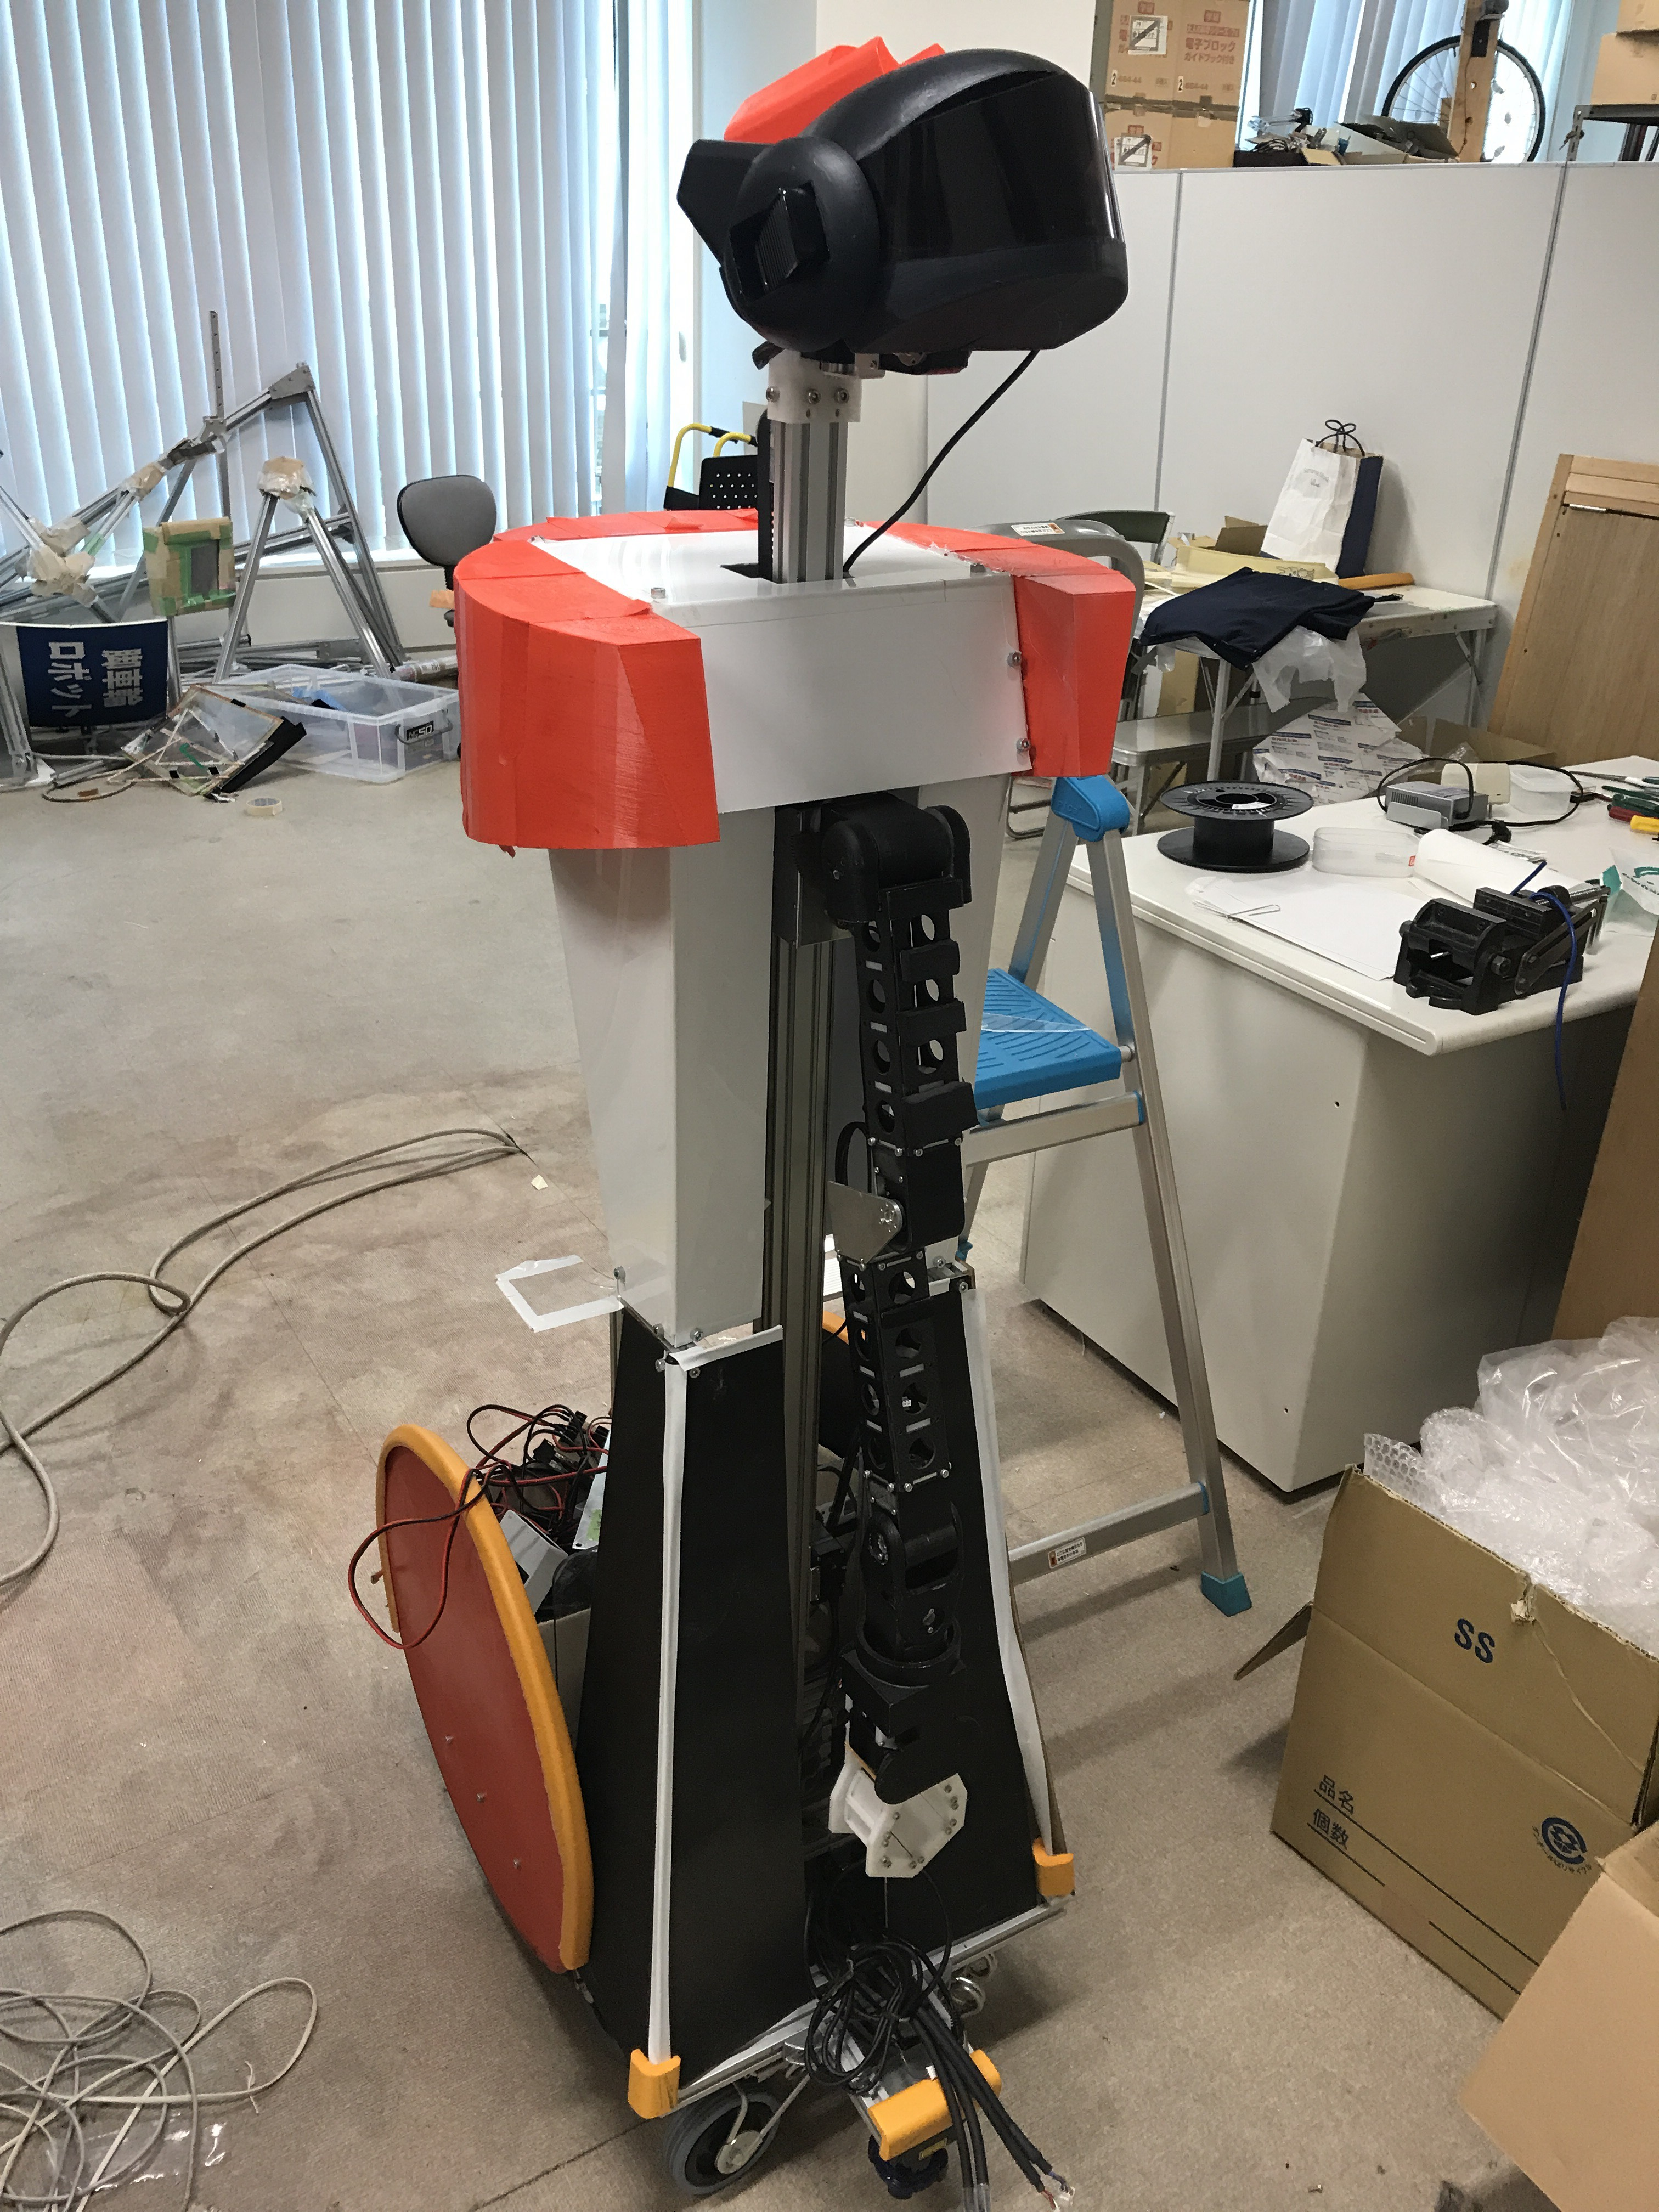
\includegraphics[width=5cm]{athome.jpg}
\caption{@home robot, hardware expected to use for this experiment}
\label{fig:home}
\end{center}
\end{figure}

\begin{figure}[!htbp]
\begin{center}
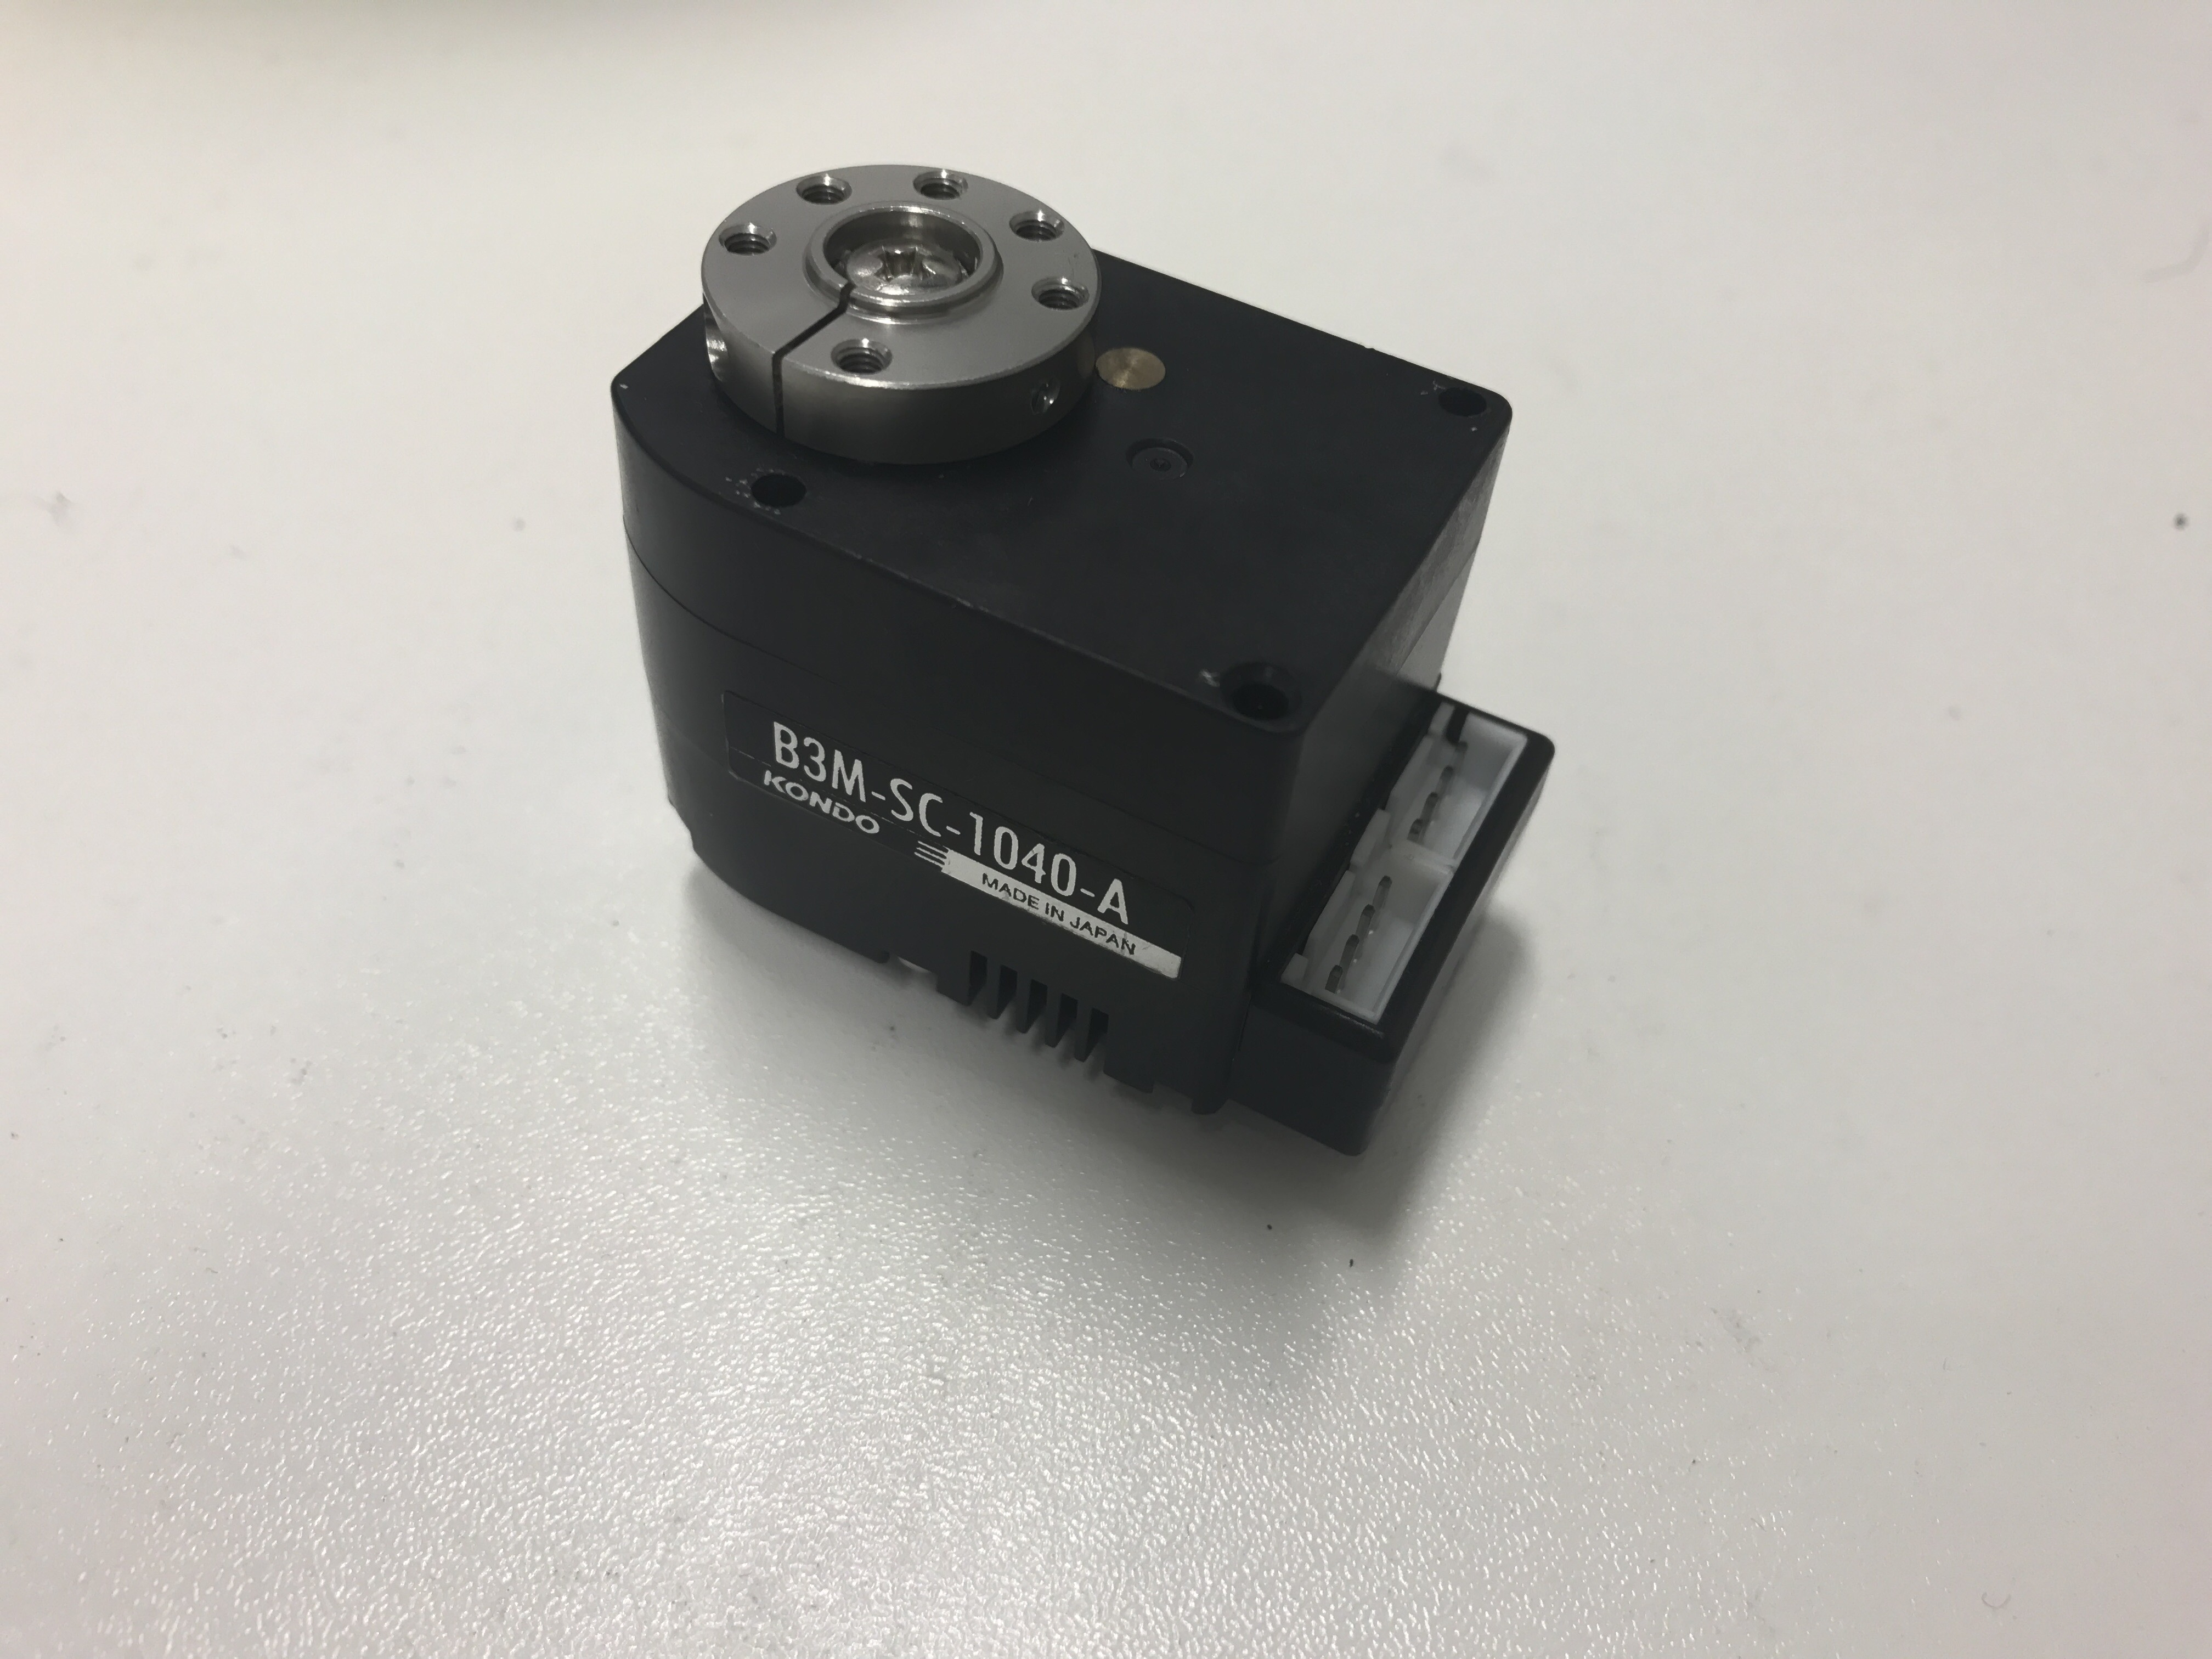
\includegraphics[width=5cm]{servo.jpg}
\caption{KONDO B3M-SC1170-A, input actuator used in manipulator}
\label{fig:servo}
\end{center}
\end{figure}

\begin{figure}[!htbp]
\begin{center}
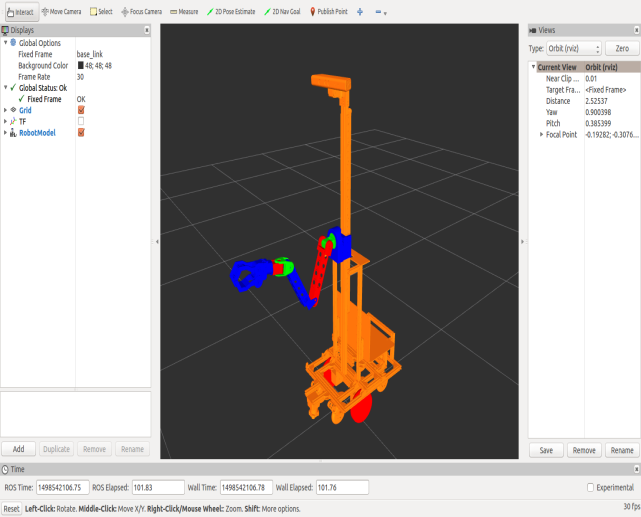
\includegraphics[width=\columnwidth]{model.png}
\caption{robot model on simulator}
\label{fig:model}
\end{center}
\end{figure}

\section{Proposed Procedure}
The first phase of the experiment will be conducted on a simulator using the robot model as shown in figure \ref{fig:model}. From the simulator, we expect to obtain the estimated data to determine the expected data on the robot and the optimal reinforcement learning parameters.

The second phase of the experiment will be conducted on the @home robot shown in figure \ref{fig:home}. Human subject guides the robot by applying adequate force to the robot arm. The experiment will examine the following conditions:

\begin{enumerate}
\item Applying force to the end-effector when the robot arm is in a fixed position.
\item Applying force to the joint when the robot arm is in a fixed position
\item Applying force to the end-effector when the robot arm is in motion
\item Applying force to the joints when the robot arm is in motion
\end{enumerate}

The direction of the force applied will parallel to robot movement, push and pull. For experiment condition 3 and 4, the robot�fs arm will move vertically every 10 second. Generating results and behavior is expected to occur every 0.1 second and the experiment will terminate when the subjects believe the robot behaves sufficiently or when 10 minutes has passed. This experiment will be expected to be performed by at least 5 subjects.
\section{Conclusion}
This paper presents an end to end method of attempting to induce a wheeled robotic manipulator using human force through reinforcement learning.

In future works it is expected to prepare an analysis on robot guidance through human force using end-to-end method.


\begin{thebibliography}{9}
\bibitem{haya}
Y. Hayashibara et al., ``Assist System for Carrying a Long Object with a Human - Analysis of a human Cooperative Behavior in the Vertical Direction -,'' Proc. 1999 IEEE/RSJ Int. Conf. on Intelligent Robots and Systems (IROS'99), 1999.

\bibitem{kosuge}
K. Kosuge, T. Hayashi, Y. Hirata, and R. Tobiyama, ``Dance partner robot -Ms DanceR-'' in IEEE/RSJ International Conference on Robots and Intelligent Systems, October 2003, pp. 345-3464.

\bibitem{yang}
Yang, Pin-Chu, et al. "Repeatable Folding Task by Humanoid Robot Worker using Deep Learning." \textit{IEEE Robotics and Automation Letters 2.2} (2017): 397-403.

\bibitem{sutton}
Sutton, R. S. and Barto, A. G. \textit{Introduction to reinforcement learning.} MIT Press, 1998.

\bibitem{mnih}
Mnih, Volodymyr, et al. "Playing atari with deep reinforcement learning." \textit{arXiv preprint arXiv:1312.5602} (2013). 

\bibitem{van}
Van Hasselt, Hado, Arthur Guez, and David Silver. "Deep Reinforcement Learning with Double Q-Learning." \textit{AAAI}. 2016.

\end{thebibliography}

\end{document}